%%%%%%%%%%%%%%%%%%%%%%%%%%%%%%%%%%%%%%%%%%%%%%%%%%%%%%%%%%%%%%%%%%%%%%%%%%%

\documentclass{standalone}

\usepackage{amsmath}
\usepackage{mathptmx}
\usepackage{pgfplots}
\usetikzlibrary{external}
\tikzexternalize{a-2-b-minus-2}
\pgfplotsset{compat=1.15}

%% IEEE uses Times Roman font, so we'll default to Times.
%% These three commands make up the entire times.sty package.
\renewcommand{\rmdefault}{ptm}
\renewcommand{\ttdefault}{pcr}
\normalfont\selectfont

\begin{document}

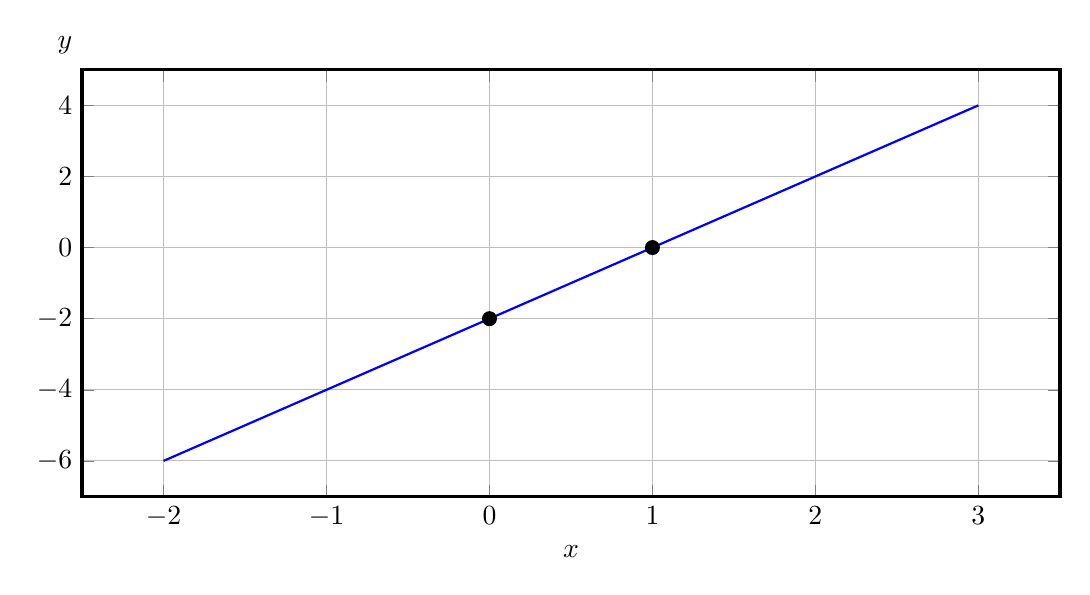
\begin{tikzpicture}
\tikzset{%%
  every mark/.append style={scale=1.0},%%
  scale=1.0%%
}
\pgfplotsset{%%
  every axis/.append style={font=\normalsize}%%
}
%%
\begin{axis}[%%
  axis line style=very thick,%%
  dotStyle/.style={only marks,mark size=2.5,black,mark color=black,mark=*},%%
  enlargelimits=true,%%
  height=7cm,%%
  plotStyle/.style={%%
    domain=-2:3,%%
    mark=none,%%
    smooth,%%
    thick%%
  },%%
  tick style={grid=major},%%
  width=14cm,%%
  %%
  %% x-axis
  xlabel={\normalsize $x$},%%
  xtick={-2,-1,0,1,2,3},%%
  xticklabels={$-2$,$-1$,$0$,$1$,$2$,$3$},%%
  %%
  %% y-axis
  every axis y label/.style={%%
    at={(axis description cs:0,1.1)},%%
    anchor=north east%%
  },%%
  ylabel={\normalsize $y$}%%
]
%%
%%
%% The function f(x) = 2x - 2.
\addplot+ [plotStyle]
{2*x - 2};
%%
\addplot[dotStyle] coordinates {
  (0,-2)
  (1,0)
};
\end{axis}
\end{tikzpicture}

\end{document}
